The bright-hidden sweep varies $c/a$ over 3.125\%, 6.25\% and 12.5\%, and separation over 6, 10, 16 and 24 bins. Each of the 12 cells contains 32 independent positive records; 96 independent single-return records provide a shared null reference. Primary amplitude and background use the ordinary-query ranges, and phase is uniform on $[14.15,16.45]$. Both methods use the common fitted full-null generator and 199 path-calibration draws. Figure~\ref{fig:power} reports all cells with 95\% Wilson intervals.

The full-bank method has a higher correct count in 12 of the 12 cells. At the nominal ratio and separation, the counts are 14/32 and 7/32. Across the specified 384-positive grid, the full and censored methods give 214 and 113 correct localizations, with 2 and 4 wrong-location reports. Their null alarms are 1 and 0 out of 96. The improvement therefore extends across the tested amplitude and separation settings.
\begin{figure*}[t]\centering
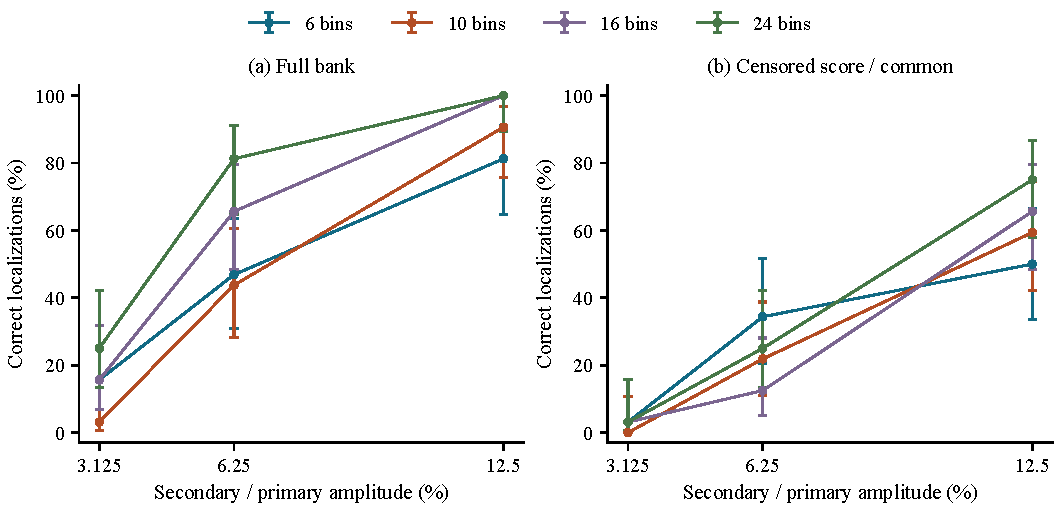
\includegraphics[width=\textwidth]{figures/fig04_power.pdf}
\caption{Correct-localization power versus secondary-to-primary incident amplitude, for four separations in the bright-hidden regime. Each point uses 32 independent two-return queries; bars are 95\% Wilson intervals. Both panels use the same query records and nominal level 0.01.}
\label{fig:power}\end{figure*}
